\documentclass[sigconf]{acmart}

\let\comment\undefined		
\usepackage{easyReview}
\usepackage{savesym}
\usepackage{xcolor}
\usepackage{booktabs}
\usepackage{multirow}
\usepackage{graphicx}
\usepackage{caption}

\newtheorem{problem}{Problem}
\usepackage{tabularx}% added for table design
\usepackage[noend]{algpseudocode}
\usepackage{tablefootnote}
\usepackage{pifont}% http://ctan.org/pkg/pifont



\newcommand{\zigzagarrow}[1]{\stackrel{\mathclap{\normalfont\mbox{#1}}}{\rightsquigarrow}}
\newcommand{\zza}[1]{\ensuremath{{\rightsquigarrow^T}}}

\newcommand{\smin}{\ensuremath{\varsigma_\textit{min}}}
\newcommand{\smax}{\ensuremath{\varsigma_\textit{max}}}
\newcommand{\cmark}{\ding{51}}%
\newcommand{\xmark}{\ding{55}}%

%% Multiline
\newcommand\CONDITION[2]%
{\begin{tabular}[t]{@{}l@{}l@{}}
		#1&#2
	\end{tabular}%
}
\algdef{SE}[WHILE]{While}{EndWhile}[1]%
{\algorithmicwhile\ \CONDITION{#1}{\ \algorithmicdo}}%
{\algorithmicend\ \algorithmicwhile}
\algdef{SE}[FOR]{For}{EndFor}[1]%
{\algorithmicfor\ \CONDITION{#1}{\ \algorithmicdo}}%
{\algorithmicend\ \algorithmicfor}
\algdef{S}[FOR]{ForAll}[1]%
{\algorithmicforall\ \CONDITION{#1}{\ \algorithmicdo}}
\algdef{SE}[REPEAT]{Repeat}{Until}{\algorithmicrepeat}[1]%
{\algorithmicuntil\ \CONDITION{#1}{}}
\algdef{SE}[IF]{If}{EndIf}[1]%
{\algorithmicif\ \CONDITION{#1}{\ \algorithmicthen}}%
{\algorithmicend\ \algorithmicif}%
\algdef{C}[IF]{IF}{ElsIf}[1]%
{\algorithmicelse\ \algorithmicif\ \CONDITION{#1}{\ \algorithmicthen}}
%% End Multiline

\usepackage{algorithm,algorithmicx}
\algnewcommand{\IIf}[1]{\State\algorithmicif\ #1\ \algorithmicthen}
\algnewcommand{\EndIIf}{\unskip\ \algorithmicend\ \algorithmicif}
\usepackage{amsmath,stmaryrd}
%% mathematics
\usepackage{braket} %% Set, tuple...
\usepackage{pifont,bigdelim}

%-%%\usepackage{amsmath,amssymb}
\newcommand{\Next}{\ensuremath{\mathbf{X}}}
\newcommand{\Globally}{\ensuremath{\mathbf{G}}}
\newcommand{\Future}{\ensuremath{\mathbf{F}}}
\newcommand{\WeakUntil}[2]{\ensuremath{{#1}\;\mathbf{W}\;{#2}}}
\newcommand{\DUntil}[2]{\ensuremath{{#1}\;\mathbf{U}\;{#2}}}
\newcommand{\MonoDeclareClause}[4]{\textsf{#1}(\texttt{#2},#3,{#4})}
\newcommand{\DeclareClause}[5]{\textsf{#1}(\texttt{#2},#3,\texttt{#4},#5)}
\newcommand{\DeclareClauseWithJoin}[6]{\textsf{#1}(\texttt{#2},#3,\texttt{#4},#5)\;\textsf{where}\;#6}
\usepackage{xspace}
\newcommand{\Sdeclare}[3]{\DeclareClause{#1}{#2}{\textbf{true}}{#3}{\textbf{true}}}
\newcommand{\LTLf}{\textup{LTL}\textsubscript{f}\xspace}
\newcommand{\xLTLf}{\texttt{xt}\textup{LTL}\textsubscript{f}\xspace}
\newcommand{\MonoDeclareClauseDataless}[2]{\textsf{#1}(\texttt{#2})}
\newcommand{\DeclareClauseDataless}[3]{\textsf{#1}(\texttt{#2}, \texttt{#3})}

\makeatletter
\newcommand{\ostar}{\mathbin{\mathpalette\make@circled\star}}
\newcommand{\make@circled}[2]{%
	\ooalign{$\m@th#1\smallbigcirc{#1}$\cr\hidewidth$\m@th#1#2$\hidewidth\cr}%
}
\newcommand{\smallbigcirc}[1]{%
	\vcenter{\hbox{\scalebox{0.77778}{$\m@th#1\bigcirc$}}}%
}
\makeatother

\usepackage{circledsteps}
\usepackage{resizegather}

\DeclareCaptionLabelFormat{andtable}{#1~#2  \&  \tablename~\thetable}

\newcommand{\gsep}{\ensuremath{\;|\;}}

\newcommand{\TopN}{\textbf{TopN Declare}\xspace}
\newcommand{\ADM}{\textbf{ADM}\xspace}
\newcommand{\ADMS}{\textbf{ADM+S}\xspace}
\newcommand{\Bolt}{\textbf{Bolt}\xspace}
\newcommand{\LogSize}{\ensuremath{ |\mathcal{L}| }}
\newcommand{\TraceLength}{\ensuremath{|\sigma|}}
\newcommand{\IF}{\textbf{IF}\xspace}
\newcommand{\CPIR}{\textbf{CPIR}\xspace}


\usepackage{xparse}
\usepackage{marginnote}
\usepackage{soul}
\usepackage{lipsum}
\usepackage{tikz}
\usetikzlibrary{calc}
\usetikzlibrary{decorations.pathmorphing}

\newlength\LineWidth
\newlength\Amplitude
\newlength\SegLength

\setlength\LineWidth{0.4pt}
\setlength\Amplitude{1pt}
\setlength\SegLength{5pt}

\definecolor{HLcolor}{RGB}{240,0,0}

% The following code contains a variation of the great code by Antal S-Z
% in his answer to http://tex.stackexchange.com/a/6029/3954
%in TeX.SX

\newcommand\tikzmark[1]{%
	\tikz[overlay,remember picture] \node (#1) {};}

\makeatletter
\newcommand{\highlight@DoHighlight}{
	\draw[HLcolor,line width=\LineWidth,decorate,decoration={zigzag,amplitude=\Amplitude,segment length=\SegLength}]  ($(begin highlight)+(0,-2pt)$) -- ($(end highlight)+(0,-2pt)$) ;
}

\newcommand{\highlight@BeginHighlight}{
	\coordinate (begin highlight) at (0,0) ;
}

\newcommand{\highlight@EndHighlight}{
	\coordinate (end highlight) at (0,0) ;
}

\newdimen\highlight@previous
\newdimen\highlight@current

\DeclareRobustCommand*\highlight[1][]{%
	\SOUL@setup
	%
	\def\SOUL@preamble{%
		\begin{tikzpicture}[overlay, remember picture]
			\highlight@BeginHighlight
			\highlight@EndHighlight
		\end{tikzpicture}%
	}%
	%
	\def\SOUL@postamble{%
		\begin{tikzpicture}[overlay, remember picture]
			\highlight@EndHighlight
			\highlight@DoHighlight
		\end{tikzpicture}%
	}%
	%
	\def\SOUL@everyhyphen{%
		\discretionary{%
			\SOUL@setkern\SOUL@hyphkern
			\SOUL@sethyphenchar
			\tikz[overlay, remember picture] \highlight@EndHighlight ;%
		}{%
		}{%
			\SOUL@setkern\SOUL@charkern
		}%
	}%
	%
	\def\SOUL@everyexhyphen##1{%
		\SOUL@setkern\SOUL@hyphkern
		\hbox{##1}%
		\discretionary{%
			\tikz[overlay, remember picture] \highlight@EndHighlight ;%
		}{%
		}{%
			\SOUL@setkern\SOUL@charkern
		}%
	}%
	%
	\def\SOUL@everysyllable{%
		\begin{tikzpicture}[overlay, remember picture]
			\path let \p0 = (begin highlight), \p1 = (0,0) in \pgfextra
			\global\highlight@previous=\y0
			\global\highlight@current =\y1
			\endpgfextra (0,0) ;
			\ifdim\highlight@current < \highlight@previous
			\highlight@DoHighlight
			\highlight@BeginHighlight
			\fi
		\end{tikzpicture}%
		\the\SOUL@syllable
		\tikz[overlay, remember picture] \highlight@EndHighlight ;%
	}%
	\SOUL@
}
\makeatother

\DeclareDocumentCommand\MarkText{O{red}O{1pt}O{5pt}m}{%
	\colorlet{HLcolor}{#1}
	\setlength\Amplitude{#2}%
	\setlength\SegLength{#3}%
	\tikzmark{endquote}\tikzmark{beginquote}\highlight{#4}%
}
\usepackage{arydshln}

\setlength{\dashlinedash}{0.2pt}
\setlength{\dashlinegap}{4.5pt}
\setlength{\arrayrulewidth}{0.2pt}
\setlength\dashlinedash{0.2pt}
\setlength\dashlinegap{1.5pt}
\setlength\arrayrulewidth{0.3pt}

%\usepackage{amsmath,amssymb}
\newcommand{\Next}{\ensuremath{\mathbf{X}}}
\newcommand{\Globally}{\ensuremath{\mathbf{G}}}
\newcommand{\Future}{\ensuremath{\mathbf{F}}}
\newcommand{\WeakUntil}[2]{\ensuremath{{#1}\;\mathbf{W}\;{#2}}}
\newcommand{\DUntil}[2]{\ensuremath{{#1}\;\mathbf{U}\;{#2}}}
\newcommand{\MonoDeclareClause}[4]{\textsf{#1}(\texttt{#2},#3,{#4})}
\newcommand{\DeclareClause}[5]{\textsf{#1}(\texttt{#2},#3,\texttt{#4},#5)}
\newcommand{\DeclareClauseWithJoin}[6]{\textsf{#1}(\texttt{#2},#3,\texttt{#4},#5)\;\textsf{where}\;#6}
\usepackage{xspace}
\newcommand{\Sdeclare}[3]{\DeclareClause{#1}{#2}{\textbf{true}}{#3}{\textbf{true}}}
\newcommand{\LTLf}{\textup{LTL}\textsubscript{f}\xspace}
\newcommand{\xLTLf}{\texttt{xt}\textup{LTL}\textsubscript{f}\xspace}
\newcommand{\MonoDeclareClauseDataless}[2]{\textsf{#1}(\texttt{#2})}
\newcommand{\DeclareClauseDataless}[3]{\textsf{#1}(\texttt{#2}, \texttt{#3})}

\makeatletter
\newcommand{\ostar}{\mathbin{\mathpalette\make@circled\star}}
\newcommand{\make@circled}[2]{%
	\ooalign{$\m@th#1\smallbigcirc{#1}$\cr\hidewidth$\m@th#1#2$\hidewidth\cr}%
}
\newcommand{\smallbigcirc}[1]{%
	\vcenter{\hbox{\scalebox{0.77778}{$\m@th#1\bigcirc$}}}%
}
\makeatother

\usepackage{circledsteps}
\usepackage{resizegather}

\DeclareCaptionLabelFormat{andtable}{#1~#2  \&  \tablename~\thetable}

\newcommand{\gsep}{\ensuremath{\;|\;}}

\newcommand{\TopN}{\textbf{TopN Declare}\xspace}
\newcommand{\ADM}{\textbf{ADM}\xspace}
\newcommand{\ADMS}{\textbf{ADM+S}\xspace}
\newcommand{\Bolt}{\textbf{Bolt}\xspace}
\newcommand{\LogSize}{\ensuremath{ |\mathcal{L}| }}
\newcommand{\TraceLength}{\ensuremath{|\sigma|}}
\newcommand{\IF}{\textbf{IF}\xspace}
\newcommand{\CPIR}{\textbf{CPIR}\xspace}


\usepackage{xparse}
\usepackage{marginnote}
\usepackage{soul}
\usepackage{lipsum}
\usepackage{tikz}
\usetikzlibrary{calc}
\usetikzlibrary{decorations.pathmorphing}

\newlength\LineWidth
\newlength\Amplitude
\newlength\SegLength

\setlength\LineWidth{0.4pt}
\setlength\Amplitude{1pt}
\setlength\SegLength{5pt}

\definecolor{HLcolor}{RGB}{240,0,0}


\newcommand\tikzmark[1]{%
	\tikz[overlay,remember picture] \node (#1) {};}

\makeatletter
\newcommand{\highlight@DoHighlight}{
	\draw[HLcolor,line width=\LineWidth,decorate,decoration={zigzag,amplitude=\Amplitude,segment length=\SegLength}]  ($(begin highlight)+(0,-2pt)$) -- ($(end highlight)+(0,-2pt)$) ;
}

\newcommand{\highlight@BeginHighlight}{
	\coordinate (begin highlight) at (0,0) ;
}

\newcommand{\highlight@EndHighlight}{
	\coordinate (end highlight) at (0,0) ;
}

\newdimen\highlight@previous
\newdimen\highlight@current


\makeatother

\DeclareDocumentCommand\MarkText{O{red}O{1pt}O{5pt}m}{%
	\colorlet{HLcolor}{#1}
	\setlength\Amplitude{#2}%
	\setlength\SegLength{#3}%
	\tikzmark{endquote}\tikzmark{beginquote}\highlight{#4}%
}
\usepackage{arydshln}

\setlength{\dashlinedash}{0.2pt}
\setlength{\dashlinegap}{4.5pt}
\setlength{\arrayrulewidth}{0.2pt}
\setlength\dashlinedash{0.2pt}
\setlength\dashlinegap{1.5pt}
\setlength\arrayrulewidth{0.3pt}




\usepackage[inline]{enumitem}
\usepackage{xfrac}
\graphicspath{ {./images/} }

\DeclareMathOperator*{\argmax}{arg\,max}
\DeclareMathOperator*{\argmin}{arg\,min}
\DeclareMathOperator*{\unif}{unif}
\DeclareMathOperator*{\dom}{dom}
%%
%% \BibTeX command to typeset BibTeX logo in the docs
\AtBeginDocument{%
  \providecommand\BibTeX{{%
    Bib\TeX}}}

%% Rights management information.  This information is sent to you
%% when you complete the rights form.  These commands have SAMPLE
%% values in them; it is your responsibility as an author to replace
%% the commands and values with those provided to you when you
%% complete the rights form.
%\setcopyright{acmcopyright}

\copyrightyear{2023}
\acmYear{2023}
\setcopyright{rightsretained}
\acmConference[GRADES \& NDA '23]{Joint Workshop on Graph Data Management Experiences \& Systems (GRADES) and Network Data Analytics (NDA)}{June 18, 2023}{Seattle, WA, USA}
\acmBooktitle{Joint Workshop on Graph Data Management Experiences \& Systems (GRADES) and Network Data Analytics (NDA) (GRADES \& NDA '23), June 18, 2023, Seattle, WA, USA}
\acmDOI{10.1145/3594778.3594881}
\acmISBN{979-8-4007-0201-3/23/06}
\usepackage{stfloats}
\usepackage{footmisc}
\usepackage{subcaption}
\algnewcommand{\LineComment}[1]{\State \(\triangleright\) #1}
\DeclareCaptionFormat{cont}{#1 (cont.)#2#3\par}

\sloppy
\begin{document}

	\title[Fast Synthetic Data-Aware Log Generation for Temporal Declarative Models]{Fast Synthetic Data-Aware Log Generation for\\ Temporal Declarative Models}

\author{Giacomo Bergami}
\orcid{0000-0002-1844-0851}
\email{Giacomo.Bergami@newcastle.ac.uk}
\affiliation{%
	\institution{Newcastle University, School of Computing}
 \city{Newcastle Upon Tyne}
	\country{United Kingdom}
}


\begin{abstract}
Business Process Management algorithms are heavily limited by suboptimal algorithmic implementations that cannot leverage state-of-the-art algorithms in the field of relational and graph databases. The recent interest in this discipline for various IT sectors (cyber-security, Industry 4.0, and e-Health) calls for defining new algorithms  improving the performance of existing ones. This paper focuses on generating several traces collected in a log from declarative temporal models by pre-emptively representing those as a specific type of finite state automaton: we show that this task boils down to a single-source multi-target graph traversal on such automata where both the number of distinct paths to be visited as well as their length are bounded. This paper presents a novel algorithm running in polynomial time over the size of the declarative model represented as a graph and the desired log's size. The final experiments show that the resulting algorithm outperforms the state-of-the-art data-aware and dataless sequence generations in business process management.
\end{abstract}


\begin{CCSXML}
<ccs2012>
   <concept>
       <concept_id>10002950.10003624.10003633.10010917</concept_id>
       <concept_desc>Mathematics of computing~Graph algorithms</concept_desc>
       <concept_significance>500</concept_significance>
       </concept>
   <concept>
       <concept_id>10003752.10003766</concept_id>
       <concept_desc>Theory of computation~Formal languages and automata theory</concept_desc>
       <concept_significance>300</concept_significance>
       </concept>
   <concept>
       <concept_id>10003752.10003809.10011254.10011256</concept_id>
       <concept_desc>Theory of computation~Branch-and-bound</concept_desc>
       <concept_significance>500</concept_significance>
       </concept>
   <concept>
       <concept_id>10003752.10003809.10011254.10011258</concept_id>
       <concept_desc>Theory of computation~Dynamic programming</concept_desc>
       <concept_significance>100</concept_significance>
       </concept>
 </ccs2012>
\end{CCSXML}

\ccsdesc[500]{Mathematics of computing~Graph algorithms}
\ccsdesc[300]{Theory of computation~Formal languages and automata theory}
\ccsdesc[500]{Theory of computation~Branch-and-bound}
\ccsdesc[100]{Theory of computation~Dynamic programming}


\keywords{Graph Automata, DFA, Synthetic Data Generator, Business Process Management}
\maketitle



\section{Introduction} 
In computer science, Business Process Management refers to the investigation of structural properties defining \textit{temporal models}; those are usually described through the subsequent occurrence of activities jointly realizing a common goal \cite{DBLP:books/sp/Weske19}.  Through these, we can check whether finite of sequences of \textit{events} of interest (\textit{traces}) conform to the model's prescriptions (\textit{conformance checking}). Procedural temporal models such as \textsc{Finite Automata} are generally less intuitive and human-readable than equivalent declarative ones summarising temporal patterns in intuitive clauses, as the size of the former is in the worst-case scenario exponential to the size of the latter \cite{ltlfnfa}. The common practitioner prefers declarative representations over procedural ones due to the possibility of enhancing and parallelising conformance-checking computations \cite{info14030173}. Procedural representations are still beneficial for efficiently generating a set of traces (\textit{logs}) conforming to a given declarative model  \cite{DBLP:conf/caise/CiccioBCM15}. The need of generating traces from procedural representations is threefold: \textit{i)} efficient probabilistic conformance starts by retrieving a set of high probability  traces conforming to a procedural model \cite{DBLP:conf/icpm/BergamiMMP21}, \textit{ii)} generating traces conforming to a given temporal model allows testing the correctness of temporal model mining algorithms \cite{DBLP:conf/caise/CiccioBCM15,DBLP:conf/ideas/ApplebyBM23}, while \textit{iii)} complex temporal  behaviours can be better represented visually by comparing similarities and differences appearing in traces \cite{8387499}.

\begin{figure}[!b]
\centering
\begin{minipage}{\linewidth}
\centering
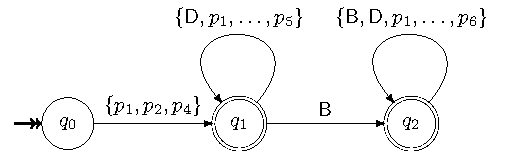
\includegraphics[scale=.7]{fig/dataaware}
\subcaption{Procedural representation of the declarative model}\label{dataawareex}
\end{minipage}

\begin{minipage}{.45\linewidth}\centering
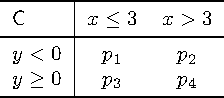
\includegraphics[scale=.8]{fig/tab1b}
\subcaption{Atoms associated to the \textsf{C}-labelled events.}\label{Clabelatom}
\end{minipage}\quad \begin{minipage}{.45\linewidth}
\centering
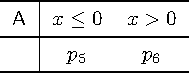
\includegraphics[scale=.8]{fig/tab1c}
\quad\\ \medskip\medskip
\subcaption{Atoms associated to the \textsf{A}-labelled events.}\label{Alabelatom}
\end{minipage}
\caption{Proceduralisation of the declarative model in Eq.\ref{eq:moddataaw}.}
\end{figure}
\begin{figure}[!t]
\centering
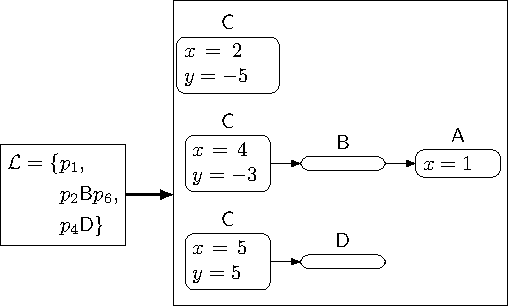
\includegraphics[scale=.7]{fig/loggenerator}
\caption{Generating a Data-Aware Log (\textit{right}) from the paths collected after traversing the procedural model in Figure \ref{dataawareex} and generating some data in compliance with the atoms defined in Figure \ref{Clabelatom} and \ref{Alabelatom}.}\label{loggenex}
\end{figure}
\begin{table*}[!t]
	\centering
\caption{Declare \textsf{templates} supported by MP-Declare Log Generator, MINERFul, and our current implementation. $A\wedge p$ ($B\wedge q$) represents the \textit{activation} (\textit{target}) condition, $A$ ($B$) denotes the activity label, and $p$ ($q$) is the data payload condition.}\label{tab:dt}
\resizebox{\textwidth}{!}{\begin{tabular}{l|p{9cm}|l}
	\toprule
	Exemplifying clause ($c_l$) & Natural Language Specification for Traces & \LTLf Semantics ($\llbracket c_l \rrbracket$)\\
	\midrule
	\textsf{Init($A,p$)} &  The trace should start with an activation & $A\wedge p$\\
	\textsf{Exists($A,p,n+1$)} & Activations should occur at least $n$ times & $\Future(A\wedge p \left[\wedge \Next (\llbracket\textsf{Exists} (A,p,n)\rrbracket)\right]_{n>0})$\\
	 %& \textsf{Absence($A,p,n+1$)}  & Activations should occur at most $n$ times & $\neg \llbracket\textsf{Exists}$($A,p,n+1$)$\rrbracket$\\
	\textsf{Precedence($A,p,B,q$)}  & Events preceding the activations should not satisfy the target & $\WeakUntil{\neg(B\wedge p)}{(A\wedge p)}$\\
	\textsf{ChainPrecedence($A,p,B,q$) }  & The activation is immediately preceded by the target. & $\Globally(\Next(A\wedge p)\Rightarrow (B\wedge q))$\\
	%& \textsf{Choice($A,p,A',p'$) }  & One of the two activation  conditions must appear. & $\Future(A\wedge p)\vee\Future(A'\wedge p')$ \\
	  \textsf{Response($A,p,B,q$) } & The activation is either followed by or simultaneous to  the target. & $\Globally((A\wedge p)\Rightarrow\Future(B\wedge q))$ \\
	  \textsf{ChainResponse($A,p,B,q$) }  & The activation is immediately followed by the target. & $\Globally((A\wedge p)\Rightarrow \Next(B\wedge q))$\\
	  \textsf{RespExistence($A,p,B,q$) }  & The activation requires the existence of the target.& $\Future(A\wedge p)\Rightarrow\Future(B\wedge q)$ \\
	 %& \textsf{ExlChoice($A,p,A',p'$) } & Only one activation condition must happen. & $\llbracket\DeclareClause{Choice}{A}{p}{A'}{p'}\rrbracket\wedge \llbracket\DeclareClause{NotCoExistence}{A}{p}{A'}{p'}\rrbracket$\\ 
	  \textsf{CoExistence($A,p,B,q$) }  & \textsf{RespExistence}, and vice versa. & $ \llbracket\DeclareClause{RespExistence}{A}{p}{B}{q}\rrbracket\wedge \llbracket\DeclareClause{RespExistence}{B}{q}{A}{p}\rrbracket$\\
	 \textsf{Succession($A,p,B,q$) }  & The target should only follow the activation. & $\llbracket\DeclareClause{Precedence}{A}{p}{B}{q}\rrbracket\wedge \llbracket\DeclareClause{Response}{A}{p}{B}{q}\rrbracket$\\

	  \textsf{ChainSuccession($A,p,B,q$) }  & Activation immediately follows the target, and the target immediately preceeds the activation. & $\Globally((A\wedge p)\Leftrightarrow\Next(B\wedge q))$\\
	 \textsf{AltResponse($A,p,B,q$) }  & If an activation occurs, no other activations must happen until the target occurs.  & $\Globally((A\wedge p)\Rightarrow(\DUntil{\neg(A\wedge p)}{(B\wedge q)}))$\\
	 \textsf{AltPrecedence($A,p,B,q$) }  & Every activation must be preceded by an target, without any other
	 activation in between &   $\llbracket\DeclareClause{Precedence}{A}{p}{B}{q}\rrbracket\wedge \Globally((A\wedge p)\Rightarrow \Next(\WeakUntil{\neg(A\wedge p)}{(B\wedge q)})$\\
	 %\midrule
	 
	 %\parbox[t]{2mm}{\multirow{2}{*}{\rotatebox[origin=c]{90}{\textit{Not.}}}} & \textsf{NotCoExistence($A,p,B,q$) } & The activation \texttt{nand} the target happen.&  $\neg(\Future(A\wedge p)\wedge\Future(B\wedge q))$\\
	 %& \textsf{NotSuccession($A,p,B,q$)} & The activation requires that no target condition should follow.& $\Globally((A\wedge p)\Rightarrow \neg\Future(B\wedge q))$ \\
	 \bottomrule
\end{tabular}}
\end{table*} 

\textit{As an example, we might be interested to encode a model prescribing that all traces start with events characterised by activities \textsc{C} (activity label) with payload values requiring that values for $x$ (or $y$) are greater than $3$ (or lower than $0$). We also allow events with activities \textsf{A} with $x$ values greater than zero only after the first occurrence of an event \textsf{B}. These two separate conditions can be described by the following data-aware model:}
\begin{equation}\label{eq:moddataaw}
\mathcal{M}=\{\textsf{Init}({\normalfont \textsf{C}},x>3\vee y< 0 ),\textsf{Precedence}({\normalfont \textsf{B}},\textbf
{true}, {\normalfont \textsf{A}},x>0)\}
\end{equation}
\textit{For generating logs conforming to such model, we first rewrite the data conditions into ``atoms'' so that each event in the trace will satisfy at most one atom condition. \tablename~\ref{Clabelatom} and \ref{Alabelatom} show the atomization result for our such a model \cite{info14030173}. We can then exploit such atoms for generating the final procedural representation of the declarative model (\figurename~\ref{dataawareex}) as per \cite{DBLP:conf/bpm/BergamiMMM21} over which traces are extracted through accepting paths; the node pointed by a free arrow remarks the initial node, while all the double-circled states remark acceptance states. Any edge $(q_i,q_j)$ associated to a set of labels $S$ is a shorthand for defining $|S|$ edges between $q_i$ and $q_j$, each of which has a distinct label in $S$. The process for transforming a declarative model into a graph via its constituent clauses is discussed in \S\ref{sec:ODFAgen}.}

\textit{By traversing such a graph (\S\ref{sec:gtrav}), we collect some paths starting from the  initial node in a set $\mathcal{L}$, which are then serialised as log traces. \figurename~\ref{loggenex} shows an example of paths starting from the initial nodes leading to acceptance states: by expanding each activity label (\textsf{B} and \textsf{C}) as an event with an empty data payload, and  each atom (e.g., $p_1$ and $p_6$) as events associated to a specific activity label (\textsf{C} and \textsf{A}) and with a data payload abiding to the definition of the atoms defined in \tablename~\ref{Clabelatom} and \ref{Alabelatom}, we can generate a data-aware traces  from a given procedural model  (\S\ref{sec:loggen}).}



It has been long established that temporal models can be used to describe good healthcare hospitalization practices \cite{Xu2020}, fluctuations in time series generated by Industry 4.0 sensors \cite{j.eswa.2022.117176}, as well as attack patterns in cyber-security scenarios \cite{info14030173}. With the ever-increasing amount of data that needs to be analysed, the ability to describe temporal models in different application contexts necessitates an urgent improvement of existing business process management algorithms, which are currently hampered by exhaustive approaches that do not utilize efficient database and graph database representations and algorithms. Such limitations are particularly evident on current state-of-the-art tools generating synthetic log from declarative temporal models. These are tampered by either inefficiently reducing the log-generation problem to a software-checking domain ({Alloy} \cite{DBLP:books/daglib/0024034}) not specifically optimised for finite models  and trace generation \cite{DBLP:conf/bpm/SkydanienkoFGM18}, or by exploiting inefficient graph algorithms for generating and traversing the resulting procedural representations \cite{DBLP:conf/caise/CiccioBCM15}. 


As our literature review shows that the trace generation problem boils down to efficiently generating a graph out of a declarative model for then traversing the resulting graph and serialising each traversed accepting path into a trace (\S\ref{sec:RW}), this paper offers an efficient solution limiting  memory occupation via tries; for reducing the visit time, we will adopt a \textsc{MinCoinChange} algorithm for combining circuits a minimum number of times with a simple path towards an accepting node so that the resulting combination satisfies the trace length requirements (\S\ref{sec:algo}). Benchmarks against the state of the art on log generation from declarative temporal models remark that our solution outperforms the state of the art (\S\ref{sec:exp}). Last, we draw our conclusions and suggest future works (\S\ref{sec:conclfut}).


\begin{figure*}[!t]
\hspace*{-.25cm}
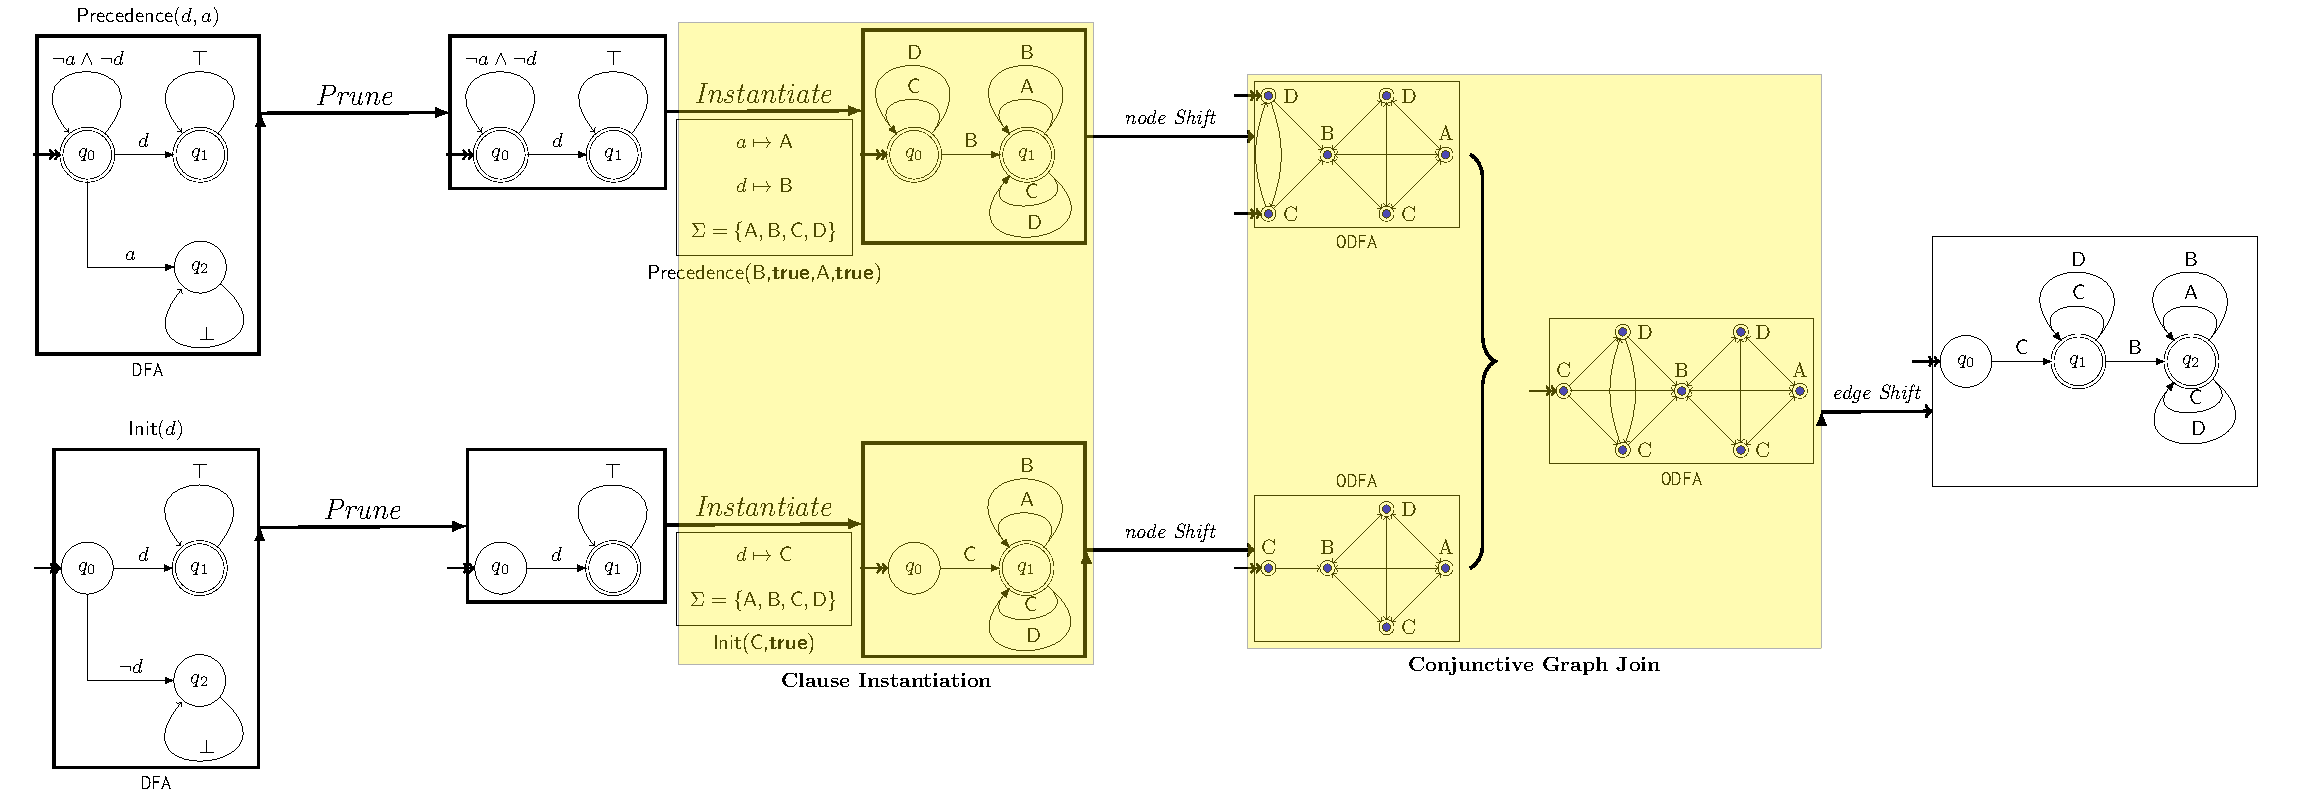
\includegraphics[width=\linewidth]{fig/transform}
\caption{Generating the procedural representation of the dataless model $\mathcal{M}=\{\textsf{Precedence}(\textsf{B},\textbf{true},\textsf{A},\textbf{true}),\textsf{Init}(\textsf{C},\textbf{true})\}$.}\label{fig:transform}
\end{figure*}
\section{Related Work}\label{sec:RW}


\paragraph*{Declare} Declarative Temporal Models can be represented using the \textit{de-facto} standard language \textit{Declare}, where each model $\mathcal{M}$ is a set of declarative clauses. Declarative temporal models are usually assessed over a finite multiset of traces $\mathcal{L}=\{\sigma^1,\dots,\sigma^m\}$ or \textit{log} \cite{info14030173}, where each (dataless) \textit{trace} $\sigma^i$ is a temporally-ordered and finite sequence of distinct events $\sigma^i=\sigma^i_1\cdots \sigma^i_n$ modelling a process run. Each event $\sigma^i_j=\braket{\textsf{A},\delta}$ is a pair, where $\textsf{A}$ is an \textit{activity label} the specific action performed/happening in a given event, and $\delta$ is a payload, i.e. a finite function mapping each key to a single value. As SQL can be expressed in terms of relational calculus, Declare can also be expressed in terms of \textit{Linear Time Logic for Finite Traces} (\LTLf) \cite{Li2020} interpreting formul\ae\, over an unbounded yet finite linear sequence of states. This logic has been recently represented in terms of algebraic operators, thus fully supporting data conditions \cite{info14030173}.  \tablename~\ref{tab:dt} provides the natural language specification for the temporal patterns associated with some templates considered in \LTLf: every single temporal pattern is expressed through \textit{templates} (i.e., an abstract parameterized property: column 1), which are then instantiated on a set of real activation, target, or correlation conditions. E.g., declarative clauses might require that a target event $\textsf{B}$ in the trace satisfying a data condition $q$ on the event's payload should immediately follow (\textsf{ChainResponse}($\textsf{A},p,\textsf{B},q$)) or precede (\textsf{ChainPrecedence}($\textsf{A},p,\textsf{B},q$)) the activation condition $\textsf{A}\wedge p$ (where \textsf{A} is the activity label and $p$ the associated data condition), that $\textsf{B}\wedge q$ might happen any time in the future after $\textsf{A}\wedge p$ (\textsf{Response}($\textsf{A},p,\textsf{B},q$)), or that $\textsf{B}\wedge q$ should never
happen before $\textsf{A}\wedge p$ (\textsf{Precedence}($\textsf{A},p,\textsf{B},q$)). If such a model contains at least one non-\textbf{true} data condition, we refer to it as \textit{data-aware}, and as \textit{dataless} otherwise.  A trace satisfies the declarative model iff. it satisfies all of its clauses. We say that the log is \textit{dataless} if each event has an empty payload, and \textit{data-aware} otherwise.


Each declarative clause containing data predicates can be represented as a single \texttt{DFA} via \LTLf \cite{FLLOAT1,ltlfnfa}, which edges represent data predicates instead of activity labels. The example in \figurename~\ref{fig:transform} (\textit{Upper left}) shows an example on how to represent \textsf{Precedence} for any possible activation condition $a$ and target condition $d$. Then, \cite{DBLP:conf/caise/CiccioBCM15} removes  all the paths not leading to an acceptance state, thus reducing the graph visiting time while avoiding that a random walk on the graph might lead to a non-acceptance state (\textit{Prune}). Last, we might freely instantiate such a graph for any activation and target condition, as well as any possible activity label \cite{DBLP:conf/bpm/BergamiMMM21} (\textit{Instantiate}). The same \figurename~ shows the instantiation of such a graph where $a$ is associated to an activation (and target) condition $\textsf{A}\wedge\mathbf{true}$ (and $\textsf{B}\wedge\mathbf{true}$) where the set of all the possible actions $\Sigma$ is a superset of the activity labels appearing in the model, e.g. $\Sigma=\{\textsf{A},\textsf{B},\textsf{C},\textsf{D}\}$. Similar considerations can be provided for data-aware models as the one in Eq.\ref{eq:moddataaw}:  to guarantee a correct graph representation,  each activation and target condition is first represented as a disjunction of mutually exclusive atoms % data conditions (\textit{atoms}), thus reducing the data-aware declarative case to the dataless one $\Sigma$
 \cite{info14030173}. This entails that atoms from \figurename~\ref{Clabelatom} satisfying the data condition in the \textsf{Init} clause are $p_1$, $p_2$, and $p_4$, while $p_6$ describes the data condition that no event shall ever satisfy before any first appearance of an event with activity label $\textsf{B}$. For this, our %we replace in 
$\Sigma$ 
consists of a superset of any activity label not associated to a table of atoms, as well as all the atoms occurring in such tables, thus $\Sigma=\{p_5,p_6,\textsf{B},p_1,\dots,p_4,\textsf{D}\}$.
%each activity label appearing in the declarative clause associated to a non-\textbf{true} data condition with all the atoms defining all the possible finite data conditions derived from the clause. 
%
 %either a target or a  associated with data predicates in our declarative model while replacing those with all the generated atoms representing all the possible 
%
%We refer the reader to \cite{info14030173} for algorithmic details concerning the atomisation process.
 

%through an \textit{atomisation} process \cite{DBLP:conf/bpm/BergamiMMM21}, where data predicates associated to a declarative models are decomposed into mutually exclusive predicates and then associated to edges' labels.


\paragraph*{Graphs} %\textit{We briefly discuss the graph data structures over which we are going to run the aforementioned algorithms, thus motivating their choice.}

\textit{Finite Automata} are edge-labelled finite-state machines that accept or reject strings of symbols based on vertex sequences (\textit{paths}) starting from the same \textit{initial vertex}. If such sequences are unique to each string, we refer to those as deterministic (DFA). Acceptance recognition is possible by visiting a graph edge whose label matches the string character to be consumed after traversal. We say that such an automaton \textit{accepts} the string if and only if the current string is empty and the current vertex is an accepting one. If we are only interested in generating graphs accepting strings, we can further simplify such automata by removing all the nodes not leading towards an acceptance state \cite{DBLP:conf/caise/CiccioBCM15}: in this scenario, we can still detect that an automaton does not accept a string if at any stage there is no edge which label matches the first character to be consumed. This improvement has two major benefits: first, we avoid scanning the rest of the string as soon as we recognise that this will be never be accepted by the automaton, and second, any path starting from the initial state and terminating on an acceptance state always returns vertex sequences corresponding to accepting strings. Our algorithm is going to leverage such optimisation for preventing the generation of paths not being accepted by the final automata. The resulting edge-labelled graphs can be converted in equivalent node-labelled automata in a linear time \cite{DBLP:conf/icpm/BergamiMMP21}: as these are the graphs allowing us to efficiently compute automata product through conjunctive graph equi-joins on the sole vertex label, we refer to those as \textit{Optimising DFA}s (ODFA).


\paragraph*{Graph Algorithms}% \textit{We considered the following existing graph algorithms thus motivating our algorithmic choices. }

The Depth-Limited-Search (DLS) algorithm is a modified version of the traditional DFS algorithm used in the iterative deepening depth-first search \cite{DBLP:journals/ai/Korf85}, which  bounds the maximum traversal depth on the graph to a given maximum depth threshold. As this algorithm always traverses the graph in depth, it does not guarantee to generate graph paths having distinct prefixes upon finishing the visit on an acceptance \texttt{DFA} state. As this will be only guaranteed by a BFS search, the present paper will therefore propose a bounded version of the BFS search, \textsc{BoundedBFS}.

Our proposed solution is also interested in computing all the simple paths between two nodes (\textsc{AllPaths}), for then arbitrarly extending those with circuits traversing those. We call a path \textit{simple} if it repeats no vertex, except that the first and last may be the same vertex. We can return such paths through an extension of the recursive implementation of DFS where the visited vertex is removed just after returning from the recursive call \cite{ASPNIST}. 


Johnson's algorithms for returning all the possible circuits in a graph \cite{doi:10.1137/0204007} allows a complete enumeration of all the possible graphs' circuits in time $O((|V|+|E|)(c+1))$, where $c$ is the total number of possible circuits within the graph. This is efficiently computed by restricting the generation of the circuits to each strong connected component of a graph while keeping tracks of the cycles being traversed. As the number of the circuits $c$ grows exponentially with the number of nodes and edges with the graph, such algorithm becomes quickly intractable for large graphs \cite{DBLP:conf/fcs/HawickJ08}. Therefore, we tolerate an approximate solution to this achievable through a simple visit of the graph through DFS, as the resulting loops will be tangent to any aforementioned simple path. 

Graph $\theta$-Joins \cite{DBLP:conf/ideas/Bergami21} are binary graph  operators returning one single graph, where each vertex in the resulting graph is the result of merging two vertices, one for each operand, matching a binary $\theta$ predicate. Different graph joins algorithms might combine edges differently. While the conjunctive join is useful to schema matching algorithms \cite{DBLP:books/sp/Melnik04}, disjunctive joins are used for merging communications networks. This paper will use conjunctive joins for the first time to speed up the computation of the product of finite state automata; the resulting automaton accepts the string iff. the same string is jointly accepted by the two original automata. %For using this algorithm, we need to shift the labels from the edges to the vertices (\textit{node Shift} in \figurename~\ref{fig:transform}) and back (\textit{edge Shift}) while guaranteeing that the resulting automata are equivalent (i.e., they accepts the same strings).



\paragraph*{Synthetic Log Generation} The synthetic log generation can be formulated as the following problem: 

\begin{problem}\label{problem}
Given a declarative model $\mathcal{M}$, we want to generate a log $\mathcal{L}$ comprising of at most $\ell$ traces of length between $\smin$ and $\smax$.
\end{problem}

\texttt{MP-Declare Log Generator}\footnote{\url{https://app.box.com/s/id6zba8nfb0krezs829vqjkpobyof5ys}} \cite{DBLP:conf/bpm/SkydanienkoFGM18} solves this problem bt reducing a temporal declarative model into a declarative specification for the Alloy Analyzer \cite{DBLP:books/daglib/0024034}, which in turn is going to generate a set of possible worlds satisfying the given constraints. The authors then convert the returned solution into a set of traces. Given that  the original paper provides no details of how such conversion is carried out and the project is closed source, we cannot provide further details on how such process is carried out. Still, the proposed approach enables the generation of traces from data-aware declarative models.

\texttt{MINERful}\footnote{\url{https://github.com/cdc08x/MINERful}} \cite{DBLP:conf/caise/CiccioBCM15} is a less recent but more documented approach on generating dataless logs. In such a model, each Declare template is associated to a regular expression where the actions corresponding to the activation and target conditions are later on instantiated for each dataless declarative clause of interest. Next, the authors generate a collection of graphs by transforming each  instantiated regular expression into a finite automata where all the states not leading to an acceptance state are removed. Then, the authors compute the product between all the previous automata using a straightforward implementation  exploiting neither indexed graph representations nor using efficient graph traversal algorithms. The authors extract the traces from such a graph by running a random walk over the composed graph with probability  $\beta=0.5$ until all of the successful traces within the desired trace length are  generated. This walk was implemented using a variation of the \textit{Iterative deepening depth-first search}. In the worst-case scenario (a fully-connected graph), the final visit has an exponential time complexity in the size of $\varsigma_\textit{max}$ and polynomial in the size of the vertices.


\section{Proposed Solution}\label{sec:algo}
As per the introduction, this paper implements\footnote{\url{https://github.com/jackbergus/gradesnda23/}}  an efficient solution to the aforementioned problem. After representing a declarative model as a graph where each label uniquely identifies a data-aware property satisfied by an event (\textit{atoms}, \S\ref{sec:ODFAgen}), we efficiently traverse the resulting graph using a novel graph traversal algorithm which is composed of two main phases: an breadth-first first visit of the graph starting from the initial state of the automaton, and a depth-first visit of the graph towards the accepting vertices while composing generated circuits and remaining simple paths (\S\ref{sec:gtrav}). Last, we convert each sequence of atoms into data-aware traces by using random value generators associated to each \textit{atom} of interest (\S\ref{sec:loggen}).


%This problem is solved through two main subsequent steps: generating a variation of a \texttt{DFA} graph (\texttt{ODFA}) out of a declarative model \S\ref{sec:ODFAgen}, efficiently traversing such automaton for generating the accepting paths from the initial node (\S\ref{sec:gtrav}), and then trasforming such paths as traces in either a tabular or in a XES format (\S\ref{sec:loggen}). 


\subsection{Proceduralisation}\label{sec:ODFAgen}
Differently from \cite{DBLP:conf/caise/CiccioBCM15}, we pre-compute each declarative template directly as a pruned \texttt{DFA} that is stored in secondary memory: \texttt{FFLOAT}\footnote{\url{https://github.com/whitemech/flloat}} \cite{FLLOAT1}  generates the graphs as in the leftmost boxes in \figurename~\ref{fig:depict}, where each edge is a propositional formula stating which are the conditions that each event must satisfy so to be consumed while traversing the edge. We then prune all the vertices not leading to an accepting states (\textit{Prune}). At warm-up, we load the pruned \texttt{DFS}s into a primary memory cache. 

Given a declarative model $\mathcal{M}$, %potentially containing data-aware clauses, 
we %first 
perform an \textit{atomisation process} for %through which we 
decomposing the data conditions associated to the activation and target conditions into a disjunction of mutually exclusive \textit{atoms} thus ensuring that each trace event will eventually satisfy at most only one of such atoms  \cite{DBLP:conf/bpm/BergamiMMM21}. We then exploit those atoms as an alphabet $\Sigma$ describing the set of all the possible labels associated to the graphs. %Due to the space limitations, we cannot provide full details of the atomisation process, for which we refer the reader to \cite{DBLP:conf/bpm/BergamiMMM21}. 
Given the atomised representation of the model, we then instantiate the activation and target conditions with the corresponding disjunction of atoms, thus instantiating each \texttt{FFLOAT} graph into a DFA (\textit{Instantiate}). 


As a 
Next, % step, 
we %want  to 
efficiently generate a single automaton accepting the strings that are jointly accepted by all the instantiated automata. For this, we need to first shift the graph labels from the edges to the vertices (\textit{node Shift}) while creating the indexing data structures required by the graph equi-join algorithm. We also map each node label to the nodes sharing the same given label. In the resulting graph, we state that a node is an accepting (initial) node if and only if this node was the result of merging together two nodes from their respective operands which were both accepting (initial) vertices. After this, we shift the labels back to the edges, as this leads to a more compact graph representation with a reduced amount of nodes (\textit{edge Shift}).

%The \texttt{ODFA} Instantiation of a Declare model $\mathcal{M}$ works as follows.
%
%\textit{First}, differently from current log generators, the \texttt{DFA} associated to each declarative template is kept in a cache and loaded at warm-up. This is possible as, differently from previously existing solutions on log generation, these \texttt{DFA} associates predicates rather than just simple activity labels to each edge, thus allowing simplifications and \cite{FLLOAT1}


%\texttt{[TODO:]} \textit{Left}, the \texttt{DFA} for \textsf{Precedence} $\neg a \mathbf{W} d$. \textit{Center}, the \texttt{A}ccepting-\texttt{DFA} prunes from the former all the paths not leading to an accepting state. \textit{Right}, instantiating the \texttt{ODFA} with an universe of symbols $\Sigma$ and with specific actions for $a$ and $d$, respectively \textsf{A} and \textsf{B}.

\figurename~\ref{fig:transform} provides an example of the proceduralisation process for a dataless declarative model. Please observe that the activity labels provided in the figure can be easily replaced with atoms through the aforementioned atomisation process. On the other hand, the generation of the procedural representation in \figurename~\ref{dataawareex} for the model in Eq.\ref{eq:moddataaw} requires first to extend $\Sigma$ as discussed in \S\ref{sec:RW}. Then, the \textit{Instantiate} of \textsf{Init} has to be rewritten considering $d\mapsto \{p_1,p_2,p_4\}$ thus requiring the generation of three distinct DFA edges, while \textit{Instantiate} for \textsc{Precedence} shall consider $d\mapsto p_6$. Overall, the more the data conditions and the more the keys being involved, the more the number of edges appearing in the graph.






\subsection{Graph Traversal}\label{sec:gtrav}
\figurename~\ref{fig:depict} summarizes the main phases defining our proposed graph traversal algorithm. This has two main phases: after choosing a node \textit{src} from which start the visit of the graph, we run a breadth-bounded version of the BFS graph visit (\textsc{BoundedBFS}, Algorithm \ref{algo:bbfs}) where the same nodes might be visited multiple times and the paths being traversed are compactly represented in main memory through a trie $T$. The visiting algorithm will stop once the trie nodes at the current maximum visit depth match the size of the log that we want to generate, $\ell$.  Next, we provide a depth traversal of the graph from the graph nodes stored at the deepest trie level towards the set of the destination nodes within the graph (\textsc{FastDepthGT}, Algorithm \ref{algo:fdgt}). The same algorithm is divided in  three distinct substeps: \textit{first}, we generate all the possible simple paths from such nodes towards the targets (\textsc{AllPaths}), \textit{second}, we use an heuristic for generating some simple circuits within the graph (\textsc{SomeCycles}), \textit{third}, we run a variation of the \textsc{Minimum Coin Change Problem} for some path $\pi$ generated by \textsc{AllPaths}, where \textit{(i)} the value associated to the coins represents the lengths of the circuits traversing $\pi$, \textit{(ii)} and the amount for which provide  the change is calculated as the number of remaining edges to be visited after visiting a trace from \textsc{BoundedBFS} and $\pi$, i.e. $|\sigma|-h_{T}(\ell)-\pi$; given this, the algorithm will return how many times a loop with a given length shall be visited so to return $\sigma$.




\begin{figure}[!t]
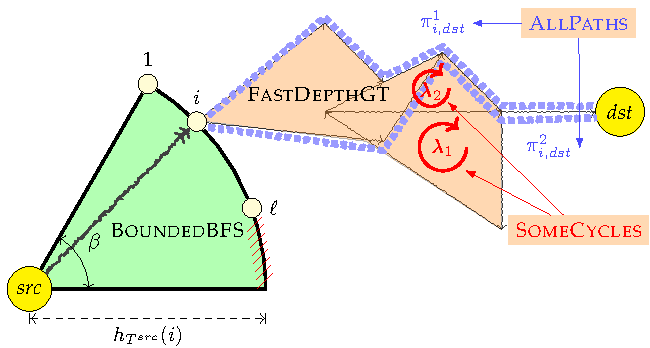
\includegraphics[width=\linewidth]{fig/algo_intuition}
\caption{Graphical depiction of the proposed algorithm: $k$ denotes the maximum path length at which we can visit at least $\ell$ nodes, $\beta$ denotes the pruning factor, $\pi_{u,v}^i$ denotes the $i$-th simple path from source $u$ to destination $v$, and $\lambda_j$ denotes a circuit in the sub-graph describing all the possible paths from $i$ to \textit{dst}.}\label{fig:depict}
\end{figure}
\begin{algorithm}[!t]
\begin{algorithmic}[1]
\Procedure{BoundedBFS}{\texttt{DFA},$T$,$\Phi_T$,$\Phi_\texttt{DFA}$;\;$\beta,\ell,\smin,\smax$}
%\ForAll{$\textit{src}\in \texttt{ODFA}.\textit{init}$}
\State $\textit{level}\gets 0$;  $X\sim \mathcal{U}_{[0,1]}$\label{loc:bfsinit}
\State $T\gets \textbf{new}\;\texttt{trie(}\texttt{DFA}.\textit{init}\texttt{);}$   \label{loc:trie}
\State $Q\gets \textbf{new}\;\texttt{queue();}$ $Q\texttt{.push(}T.\textit{root}\texttt{)}$; \label{loc:justroot}
 \State $\Phi_{T}\gets\emptyset$; $\Phi_\texttt{DFA}\gets\emptyset$\label{loc:levelnodes}
\While{$Q\neq\emptyset$}
\State \textit{ptr}$\gets Q.\texttt{pop();}$
\If {$h_T(\textit{ptr})>\textit{level}$} 
\State $\textit{level}\gets h_{T}(\textit{ptr})$; $\Phi_{T}\gets\emptyset$; $\Phi_\texttt{DFA}\gets\emptyset$;\label{loc:bfsclear}
\EndIf
\State
 $\Phi_{T}\gets\Phi_{T}\cup\{\textit{ptr}\};$ $\Phi_\texttt{DFA}\gets \Phi_\texttt{DFA}\cup\{\textit{ptr}.\texttt{node}\}$\label{loc:bfsupd}

\State \algorithmicif\ $|\Phi_\texttt{DFA}|=\ell+1$ \algorithmicthen\ \textbf{break}\label{loc:bfsthenbreak}
\If{$h_{T}(\textit{ptr})\leq \smax$}\label{loc:bfsupper}
\If{$\textit{ptr}\texttt{.node}\in\texttt{DFA}.\textit{accept}$ \textbf{and} $h_{T}(\textit{ptr})\geq \smin$}
\State $\mathcal{L}\gets \mathcal{L}\cup\{ T\textit{.root}\texttt{.node}\zza{T}\textit{ptr}\texttt{.node}\}$\label{loc:newdata}
\State $\ell\gets\ell-1$
\State \algorithmicif\ $\ell=0$ \algorithmicthen\ \Return $\mathcal{L}$\label{loc:bfsbreakcongruo}
\EndIf
\ForAll{\textbf{unique} $e\sim \unif\{\texttt{DFA}.\textit{out}(\textit{ptr}\texttt{.node})\}$}

\If{$\mathbb{E}[X]\geq \beta$}
\State $ptr'\gets T.\texttt{addChildTo}(e.\texttt{dst}\xrightarrow{e}\textit{ptr})$\label{loc:addchild}
\State $Q.\texttt{push}(\textit{ptr}')$\label{loc:bfsnext}
\EndIf
\EndFor

\EndIf
\EndWhile

%\EndFor
\EndProcedure
\end{algorithmic}
 \caption{Generating distinctive trace prefixes, $O(\ell)$.}\label{algo:bbfs}
\end{algorithm} 
\paragraph*{\textsc{BoundedBFS}}

Algorithm \ref{algo:bbfs} starts the visit of the \texttt{DFA} from its sole source node \texttt{DFA}.\textit{init}. We count the visiting depth levels of the graph starting from zero so that the number of depth levels reflects the number of traversed edges, and we initialize a pseudo-random number generator with uniform distribution in the interval $[0,1 ]\subseteq\mathbb{R}^+$ (L. \ref{loc:bfsinit}). A trie tracks the traces' prefix  generated from the source node (L. \ref{loc:trie}), thus remembering which edge was traversed to reach a given node (L. \ref{loc:addchild}). Differently from customary BFS algorithms directly enqueueing graph nodes, our queue  stores trie nodes encompassing both path and graph node information (L. \ref{loc:justroot}). We also use roaring bitmaps \cite{WangLPS17} for representing a collection of distinct trie pointers ($\Phi_T$) and distinct graph nodes pertaining to the current maximum visiting level ($\Phi_\texttt{DFA}$, L. \ref{loc:levelnodes}). We update such levels once new nodes pertaining of the same level of depth are visited (L. \ref{loc:bfsupd}) and completely cleared once a new depth level is visited (L. \ref{loc:bfsclear}). 

The $\ell$ parameter states the maximum number of traces to be generated while visiting the graph. If at the current level we start exceeding the given amount, we then break the iteration (L. \ref{loc:bfsthenbreak}). Similarly, we continue to traverse the graph from that point only if traversing a new edge will not increase the trace length above the given maximum trace threshold (L. \ref{loc:bfsthenbreak}). At this point, we might consider all the paths from this point on the trie backwards as a candidate trace (L. \ref{loc:newdata}) if and only if the current state is an acceptance state which is above the minimum trace length threshold $\smin$. We can also stop the iteration once we already visited an adequate amount of paths for generating such traces (L. \ref{loc:bfsbreakcongruo}). We progress the graph visit only if we need to generate more traces: for any currently visited node we random sample the next nodes from the $n$ outgoing edges from the current node while guaranteeing that the actually visited ones are $\beta n\leq n$ with $\beta$ a probability value; after traversing the edge, we extend the trie (L. \ref{loc:addchild}) and progress the graph visit with the adjacent node (L. \ref{loc:bfsnext}). 


%As a \texttt{DFA} guarantees the absence of more than one outgoing edge from the same node with the same label, by guaranteeing that any traversal algorithm will visit each edge at most once each time a vertex is met will guarantee to generate distinct labels out of each node. Therefore, our bounded BFS visit also guarantees the generation of distinct prefixes within the same prefix length, thus resolving into the generation of distinct traces. Given the size of the alphabet $|\Sigma|$ as the maximum possible branching factor of the graph, in the worst case scenario this algorithm runs in $\sum_{d=1}^h|\Sigma|^d$ which is in $O(|\Sigma|^h)$ time; given $h$ the deepest level of the visit for which the algorithm generates $\ell$ unique prefixes, thus $|\Sigma|^h=\ell$, we state that this first phase runs in linear time with respect to the expected log size $\ell$ to be returned, $\mathcal{L}$. Therefore, we can state that this phase reaches the algorithmic optimality, as the time required to visit the graph matches the number of the traces to be generated regardless of their final length.






%%%%%%%%%%%%%



\paragraph*{\textsc{FastDepthGT}}    Algorithm \ref{algo:fdgt} extends the path prefixes conveniently stored in our trie by generating the remaining $\ell$ paths left our from our previous phase for each of the distinct nodes at the previous maximum visiting depth.
This phase  is run only if the previous phase has not returned an adequate amount of traces. Such algorithm also guarantees that, if the computation is terminated while providing less that the number of the expected traces, this always returns the maximum number of accepting traces generable within the given minimum and maximum trace length bounds.
 This novel step implements a single-source multi-target visit of the graph, where the single source is each of the aforementioned nodes and the targets are all the accepting vertices of the graph. In order to reduce the graph visiting cost as much as possible, we want to visit each circuit appearing in the graph at most once, while guaranteeing the generation of the traces within the length range of interest. 


\begin{algorithm}[!t]
\begin{algorithmic}[1]
\Procedure{FastDepthGT}{\texttt{DFA},$T$,$\Phi_T$,$\Phi_\texttt{DFA}$;\;$\beta,\ell,\smin,\smax$}
\State $\Lambda\gets$\Call{SomeCycles}{\texttt{DFA}}\label{sec:somecycle}
\State $M(u)\gets \{\lambda\in \Lambda|u\in\lambda\}$ \textbf{for} $u\in \texttt{DFA}.\textit{V}$\label{loc:subset}
\ForAll{$\textit{ptr}\in \Phi_{T}$}
\State $i\gets\textit{ptr}\texttt{.node}$;  $h\gets h_{T}(\textit{ptr})$
\State $\varpi\gets T\textit{.root}\texttt{.node}\zza{T}\textit{ptr}\texttt{.node}$\label{loc:varpidef}
\ForAll{$\pi\in $ \Call{AllPaths}{$i$,\,\texttt{DFA}.\textit{accept}} \textbf{s.t.} $|\pi|\leq \smax-h$}
\State $\pi'\gets\pi\circ\varpi$
\If{$|\pi|\geq \smin-h$}
\State $\mathcal{L}\gets \mathcal{L}\cup \{\pi'\}$; $\ell\gets\ell-1$\label{loc:retinbound}
\Else
\State $L(n)\gets \{\lambda \in \Lambda|\;|\lambda|=n,\lambda\cap\pi\neq\emptyset\}$
\ForAll{$\smin\leq j\leq \smax$ \textbf{s.t.} $j-|\pi'|>0$}
\State \textit{sol}$\gets$\Call{MinCoinChange}{$\dom(L),j-|\pi'|$}
\If{\textit{sol}$\neq\emptyset$}
\ForAll{$\braket{\textit{coin},\textit{times}}\in\textit{sol}$}\label{loc:EachSolLine} %,\textit{coin}\in\dom(L)
\State $\lambda\gets \texttt{choice}(L(\textit{len}))$
\State $n\gets \texttt{choice}(\lambda\cap \pi)$
\State $\lambda'\gets\lambda[n:]\circ\lambda[:-n]$
\State $\pi'\gets \pi'[:-n]\circ \left(\bigcirc^\textit{times}\lambda'\right)\circ \pi'[n:]$\label{loc:expansion}
\EndFor
\State $\mathcal{L}\gets\mathcal{L}\cup\{\pi'\}$; $\ell\gets\ell -1$; \textbf{break}\label{loc:newtracegen}
\EndIf
\EndFor
\EndIf
\State \algorithmicif\ $\ell=0$ \algorithmicthen\ \Return $\mathcal{L}$ \label{loc:sectermcond}
\EndFor
\EndFor
\State \Return $\mathcal{L}$\Comment{\textit{We generated less traces than required}}
\EndProcedure
\end{algorithmic}
 \caption{Fast Depth Graph Traversal}\label{algo:fdgt}
\end{algorithm}
After storing some cycles in $\Lambda$ as discussed in \S\ref{sec:RW} (L. \ref{sec:somecycle}), we associate to each node in the graph a subset of cycles $\Lambda$ containing such a node (L. \ref{loc:subset}). To minimise the number of graph visits, we sample the accepting paths $\pi$ for each distinct graph node $i=$\textit{ptr}.\texttt{node} associated to a trie leaf ($\Phi_T$) providing a path $\varpi$ from the source \textit{src} of length $h$ (L. \ref{loc:varpidef}). We add the resulting  concatenated path $\pi'\gets\pi\circ\varpi$ to the solutions in $\mathcal{L}$ if its length is within the boundaries of minimum and maximum trace length (L. \ref{loc:retinbound}). Otherwise, we try to extend $\pi'$ with some circuits incident to it. To do so, we run the \textsc{MinCoinChange} algorithm for determining how many times we need to extend $\pi'$ with the loops in $\Lambda$ incident to $\pi$ so to generate a trace within the minimum and maximum trace length bounds. For doing so, we consider the lengths of such loops as the coins' values, while the amount of money $j-|\pi'|$  for each $j\in [\smin,\smax]$ represents the number of edges to be visited for returning the trace. The solution of the \textsc{MinCoinChange} problem will then return us the minimum amount of \textit{times} we need to traverse a circuit of a given length (\textit{coin}) so to finally reach the desired trace length (L.\ref{loc:EachSolLine}). We choose one circuit among all of the possible incident circuits to the current simple path and expand it on the path the desired amount of times (L.\ref{loc:expansion}). After this, we put the expanded path in the set of all the possible logs (L.\ref{loc:newtracegen}). We terminate as soon as we reach the desired log size (L.\ref{loc:sectermcond}).

 
%As the \textsc{MinCoinChange} problem has a time complexity of $O(nv)$ for $n$ coins when the value to give the rest is $v$, given that in the worst case scenario  simple paths have length $|V|-\ell$ and circuits have a length of at most $|V|$, its time complexity such algorithm over such graphs is at most quadratic in the size of the nodes. In the worst case scenario, such algorithm is also run at most $\varsigma_\textit{max}-\varsigma_\textit{min}$ times. Despite the number of all the possible simple paths in a graph is at most $|V|!$, the algorithm ensures that we stop the iteration as soon as we find $\ell$ paths. As each DFA generated by the declarative clause guarantees that there exists at least one circuit of length one for each simple path, we can then freely assume that under our specific assumptions the algorithm will run in at most a number of polynomial steps on the size of the output as it will have a time complexity of $O( |V|^2 \ell (\varsigma_\textit{max}-\varsigma_\textit{min}))$.



\subsection{Log Serialisation}\label{sec:loggen}
At this stage, the log being generated is dataless, where each event is only remarked by its activity label that, at this stage, only represents an atom (i.e., the activity label and data condition) that an event should satisfy. To generate the payload from these events, we generate strings and numbers within the ranges specified by the atoms via random generators. For strings, we restrict our interest to the ones having an ASCII representation. Last, we serialize the log in either a XES format or in a tab separated format, where the payload conditions associated to the events are dropped. The latter implementation is merely provided for a fair comparison with the \texttt{MINERful} generator which correctly supports such representation, while XES is used in compliance to the log format returned by \texttt{MP-Declare Log Generator}.

\section{Experimental Analysis}\label{sec:exp}
Our benchmarks exploited a Dell Mobile Precision Workstation 5760 on Ubuntu 22.04: Intel® Xeon(R) W-11955M CPU @ 2.60GHz $\times$ 16, 64GB DDR4 3200MHz RAM, 500 GB of free disk space. We generated four declarative models of increasing number of clauses (from 2 to 8), where the $i$-th model is always a subset of the $i+1$-th one. For a better comparing our system with both \texttt{MINERful} generating dataless logs and
\texttt{MP-Declare Log Generator} generating data-aware ones, we generated both a data-aware and a dataless version of the declarative models by first generating the data-aware models; the dataless ones are generated by replacing in the formerthe data conditions in the former with \textbf{true} predicates. The resulting datasets for both our implementation and the competing approaches are freely available\footnote{\url{https://osf.io/2pmvs/}}. After benchmarking our proposed solution in proceduralisation and graph traversal times (\S\ref{ssec:proposed}), we separatedly compare \texttt{MINERful} against our solution with a dataless model (\S\ref{ssec:dataless}) as well as \texttt{MP-Declare Log Generator} against our solution with a data-aware model (\S\ref{ssec:dataaware}). As the competing solutions can neither provide benchmarking times for the sole graph traversal algorithm nor disable the serialisation of the returned traces to disk thus limiting the overall running time, we compare their overall running time with our ours. This last analysis will remark that the running time is heavily bounded by the serialisation time.


\begin{table}[!t]
\centering
\caption{Model proceduralisation time ($t_p$) in milliseconds.}\label{tab:proceduralisation}
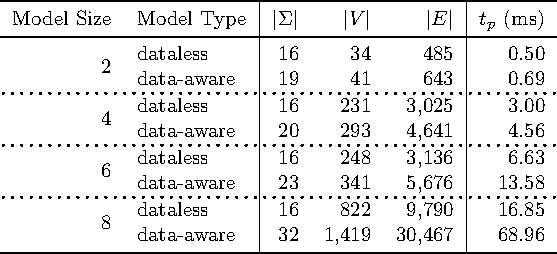
\includegraphics[scale=.7]{fig/tabmod}
\end{table}
\subsection{Benchmarking the Proposed Solution}\label{ssec:proposed}


\textit{Proceduralisation time.} \tablename~\ref{tab:proceduralisation} shows the running time required to transform a declarative model into its propositional counterpart. Results are provided for both the dataless and the data-aware model. As this phase is independent of the log parameters, we are only interested in comparing the time required to generate a procedural model out of the declarative one ($t_p$) against the set of the overall $\Sigma$ associated with the graph, as well as the number of nodes $|V|$ and edges $|E|$ associated to the returned graph. $t_p$ considers the time to instantiate the graphs as stored in the cache,  the node shift for each instantiated graph,  the conjunctive graph join across those, and the edge shift on the resulting joined graph. Our analysis showed a stronger correlation between running time and the number of edges ($p\geq 0.99$) while the correlation with the number of atoms and model size is quite limited. This remarks that the instantiation process as well as the multi-graph-join step is heavily bounded by the number of edges in each single graph. Results show an almost linear correlation between the size of the resulting graph's edge $|E|$ with the overall running time, thus showing optimal algorithmic time.\medskip

\begin{figure}[!t]
\centering
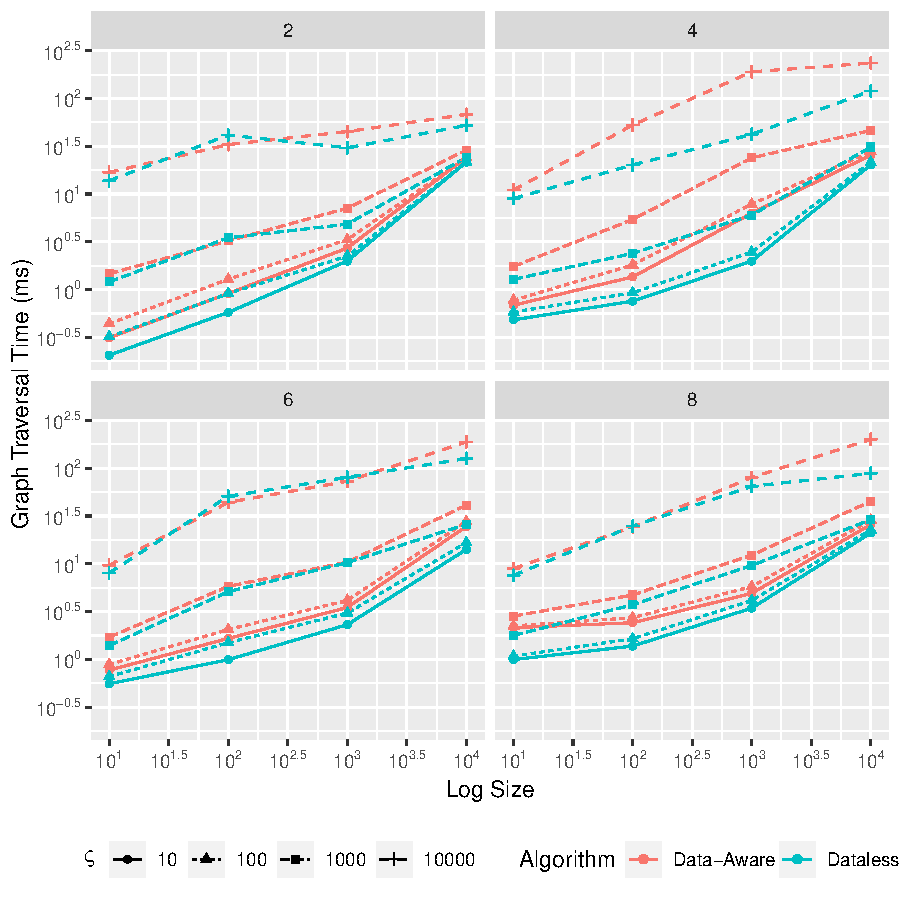
\includegraphics[width=\linewidth]{fig/TraversingTimesSolo}
\caption{Graph Traversal times in milliseconds grouped by model size. Colours differentiate different types of models, while line style and symbol shape reflect different trace lengths ($\varsigma_\textit{min}=\varsigma_\textit{max}=\varsigma$).}\label{traversetimesolo}
\end{figure}
\textit{Graph Traversal.} We analysed the running times for traversing the graphs resulting from the previous phase: we wanted then to generate logs of different sizes and growing with a tenfold increase ($|\mathcal{L}|=\ell$ and $\ell\in{10^1,10^2,10^3,10^4}$); to provide more legible plots, we constrained the minimum $\varsigma_\textit{min}$ and maximum $\varsigma_\textit{max}$ trace length to the same value $\varsigma$, also growing by a tenfold increase ($\varsigma\in\{10^1,10^2,10^3,10^4\}$). We kept the random edge sample factor to $\beta=.9$ and tested our algorithm on both dataless and data-aware models. \figurename~\ref{traversetimesolo} shows that,  in the best case scenario, traversing automata generated from dataless models is faster than traversing ones generated from data-aware ones, as the former have usually a smaller size than the others while, in the worst case scenario, they exhibit comparable running times. We can also observe that running times are heavily affected by the trace length of the results to be provided: this is more evident while going from $\varsigma=10^3$ to $\varsigma=10^4$, where we remark a tenfold increase in running time. Such discrepancy becomes less evident at inferior trace length increases. Running times are also polynomial on the size of the desired log size. Model sizes influence the running times only when smaller logs are returned, while desired log sizes influence the running times otherwise. Our implementation gives fast graph traversal in less than one second. 
 
\begin{figure}[!t]
\centering
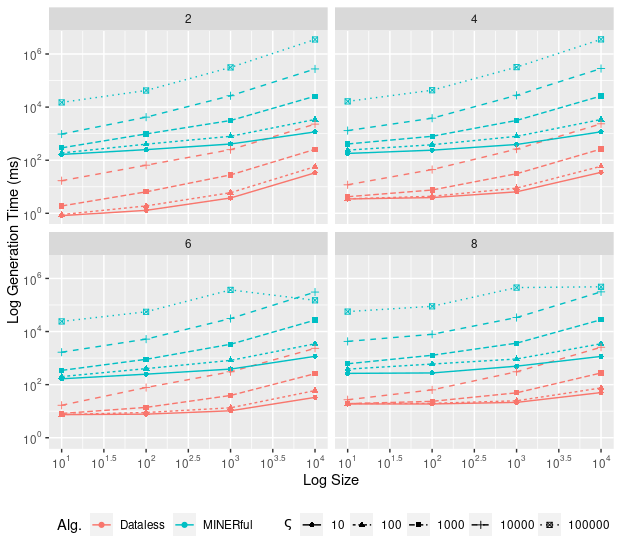
\includegraphics[width=\linewidth]{fig/Minermer.png}
\caption{Complete Log Generation Time for dataless declarative models, grouped by model size.}\label{dataless}
\end{figure}
\subsection{Dataless Log Generation}\label{ssec:dataless}
Results in \figurename~\ref{dataless} compare the full log generation time for both our solution with a dataless model and \texttt{MINERful}, also accepting dataless models in a specific \texttt{JSON} format. Our aformentioned dataset provides the \texttt{JSON} representation required for such generator. To enhance algorithms' performances, we serialise their resulting logs in a tabular separated format. Our solution constantly outperforms \texttt{MINERful} by at least one order of magnitude. This difference is even more remarkable for longer traces and larger logs, where our solution can be at most two orders of magnitudes more performant than our competitor. As the serialisation into a simplistic format annihilate any potential overhead from verbose XES serialisation, longer running times might be only be ascribed by the underperforming algorithms being choose for either traversing the graph or generating the graph to be traversed out of each declarative clause. As the tool does not provide further running times for each specific phase, we cannot further ascertain which might be the primary cause of this overhead. Last, by comparing our tools' overall running time with the graph traversal and model proceduralisation phases, we can clearly remark that the overall running time is heavily dominated by the serialisation of the generated log in secondary memory.

\begin{figure}[!t]
\centering
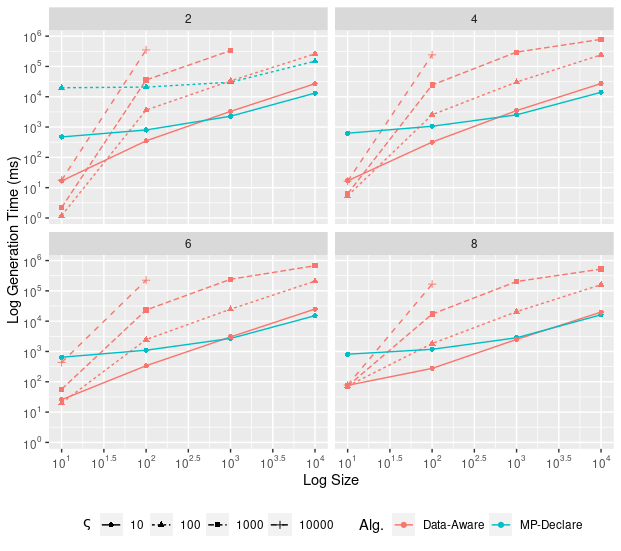
\includegraphics[width=\linewidth]{fig/Datamer.png}
\caption{Complete Log Generation Time for data-aware declarative models, grouped by model size.}\label{dataware}
\end{figure}
\subsection{Data-Aware Log Generation}\label{ssec:dataaware}
Results in \figurename~\ref{dataware} leverage the same experimental setting as in the previous paragraph: both \texttt{MP-Declare (Log Generator)} and our proposed solution considered data-aware models. We stopped running both generators when they run for more than $10^6$ milliseconds. Both generators were set to serialise the log in XES format. Our competitor can only efficiently generate data when traces are considerably short ($\varsigma=10$). Given that our solution was able to serialise the log in less than $10^6$ ms, despite taking more time than serialising an equivalent amount of data in a tab-separated format (cfr. \figurename~\ref{dataless}), this remarks that our competitor spends most of the time running the Alloy generator for which extract data-aware traces. These experiments remark on the superiority of the graph-based approach for log generation if compared to non-graph-based approaches (\texttt{MP-Declare}).

\section{Conclusions and Future Works}\label{sec:conclfut}
This paper presented a novel solution for generating data-aware and dataless logs out of declarative models. After converting such models into ``pruned'' finite state automata, our solution reaps the benefit of state-of-the-art binary graph operators while proposing a novel algorithm for efficiently traversing those generated graphs. Our solution outperforms existing state-of-the-art log generators from the Business Process Management domain, both generating a sample of log traces from the procedural model representation and exploiting heuristics for engaging with the graph traversal (e.g., random walks).

Future works will assess the compatibility of the graphs generated by FLLOAT with its newer version, \texttt{logaut}\footnote{\url{https://github.com/whitemech/logaut}}, and will assess different possible initial graph representations for \LTLf formul\ae~ as a basis for trace generations. Also, an extension of the graph traversal algorithm to any possible graph representation will require changing the algorithm for returning the circuits in the graph so as not to rely on structural properties of procedural models generated from declarative ones, such that the existence of at least one circuit over one single graph node. Our future endeavours will be therefore directed at finding better heuristics for generating some circuits occurring in the graph. We will also investigate the possibility of extending such a solution by supporting declarative clauses expressing data correlation conditions between activated and targeted events.  Future experiments will be performed to better compare the adequacy and quality of the traces generated by the different generators which, however, must fulfil the requirements of the time model. Last, we will also consider defining novel data representations for data-aware logs significantly improving the data serialisation time to disk, thus attempting to further improve the running time of the overall solution.


\bibliographystyle{ACM-Reference-Format}
\bibliography{refs.bib}


\end{document}
\endinput
%%
%% End of file `sample-sigconf.tex'.
